\documentclass{article}
\usepackage[margin=0.9in]{geometry}
\usepackage[utf8]{inputenc}

% Get better typography
\usepackage[protrusion=true,expansion=true]{microtype}  
% For algorithms
\usepackage[boxruled,linesnumbered,vlined,inoutnumbered]{algorithm2e}
\SetKwInOut{Parameter}{Parameters}
% For basic math, align, fonts, etc.
\usepackage{amsmath}
\usepackage{amsthm}
\usepackage{amssymb}
\usepackage{mathtools}
\usepackage{mathrsfs}
\usepackage{rotating}
\usepackage{soul}
\usepackage{gensymb} % For \degree
\usepackage{lscape}
% For \thead to make line breaks in tables
\usepackage{array}
\usepackage{makecell}
\renewcommand\theadalign{bc}
\renewcommand\theadfont{\bfseries}
\renewcommand\theadgape{\Gape[4pt]}
\renewcommand\cellgape{\Gape[4pt]}
\usepackage{courier} % For \texttt{foo} to put foo in Courier (for code / variables)
\usepackage{lipsum} % For dummy text
% For images
\usepackage{graphicx}
\usepackage{subcaption}
\usepackage[space]{grffile} % For spaces in image names
% For bibliography
\usepackage[round]{natbib}
% For color
\usepackage{xcolor}
\definecolor{light-grey}{rgb}{0.9,0.9,0.9}
\definecolor{dark-red}{rgb}{0.4,0.15,0.15}
\definecolor{dark-blue}{rgb}{0,0,0.7}
\usepackage{environ}
% Only show sections in table of contents and rename
\setcounter{tocdepth}{2}
\renewcommand{\contentsname}{Table of Contents}
% For links (e.g., clicking a reference takes you to the phy)
\usepackage{hyperref}
\hypersetup{
    colorlinks, linkcolor={dark-blue},
    citecolor={dark-blue}, urlcolor={dark-blue}
}

\newcommand{\TODO}[1]{\textcolor{blue}{\textbf{{#1}}}}
\newcommand{\WARNING}[1]{\textcolor{red}{\textbf{{#1}}}}
\newcommand{\POINTS}[1]{\textcolor{purple}{\textbf{{#1}}}}

\begin{document}


%-----------------
%   Homework 5
%-----------------
\newpage
\begin{center}
    \begin{Large}
    CMPSCI 687 Homework 5 - Fall 2022
    \end{Large}
    \\
    Due November 25, 2022, 11:55pm Eastern Time
\end{center}
\addcontentsline{toc}{subsection}{\textbf{Homework 5}}



\section{Instructions}

This homework assignment consists only of a programming portion. While you may discuss problems with your peers (e.g., to discuss high-level approaches), you must write your own code from scratch. The exception to this is that you may re-use code that you wrote for the previous homework assignments. \textbf{We will run an automated system for detecting plagiarism. Your code will be compared to the code submitted by your colleagues, and also with many implementations available online.} In your submission, do explicitly list all students with whom you discussed this assignment. Submissions must be typed (handwritten and scanned submissions will not be accepted). You must use \LaTeX. The assignment should be submitted on Gradescope as a PDF with marked answers via the Gradescope interface. The source code should be submitted via the Gradescope programming assignment as a .zip file. Include with your source code instructions for how to run your code. You \textbf{must} use Python 3 for your homework code. You may not use any reinforcement learning or machine learning-specific libraries in your code, e.g., TensorFlow, PyTorch, or scikit-learn. You \textit{may} use libraries like numpy and matplotlib, though. The automated system will not accept assignments after 11:55pm on November 25. The tex file for this homework can be found \href{https://people.cs.umass.edu/~bsilva/courses/CMPSCI_687/Fall2022/HWs/HW5_Source.zip}{here}.


\begin{center}
    \WARNING{Before starting this homework, please review this course's policies on plagiarism by  \\reading Section 10 of the \href{https://people.cs.umass.edu/~bsilva/courses/CMPSCI_687/Fall2022/F22_687_Syllabus_v2.pdf}{\textcolor{red}{\underline{syllabus}}}.}
\end{center}

\noindent\rule{\textwidth}{1pt}

\vspace{0.2cm}
\section*{Programming Assignment \POINTS{[100 Points, total]}}

In this assignment, you will implement three algorithms based on Temporal Difference (TD): TD-Learning for policy evaluation; SARSA; and Q-Learning. You will deploy all three algorithms on the 687-Gridworld. You will also deploy SARSA and Q-Learning on the Mountain Car domain. \textbf{Notice that you may \ul{not} use existing RL code for this problem---you must implement the learning algorithms and the environments entirely on your own and from scratch.} The complete definition of the 687-GridWorld domain can be found in Homework 3. The complete definition of the Mountain Car domain can be found in Homework 2.

\vspace{0.15in}
General instructions:


\begin{itemize}
    \item You are free to initialize the $q$-function in any way that you want. More details about this later. 
    \item Whenever displaying values (e.g., the value of a state), use 4 decimal places; e.g, $v(s)=9.4312$.
    \item Whenever showing the value function and policy learned by your algorithm, present them in a format resembling that depicted in Figure \ref{fig:v_pi_star}.
\end{itemize}

\begin{figure}[!ht]
    \centering
    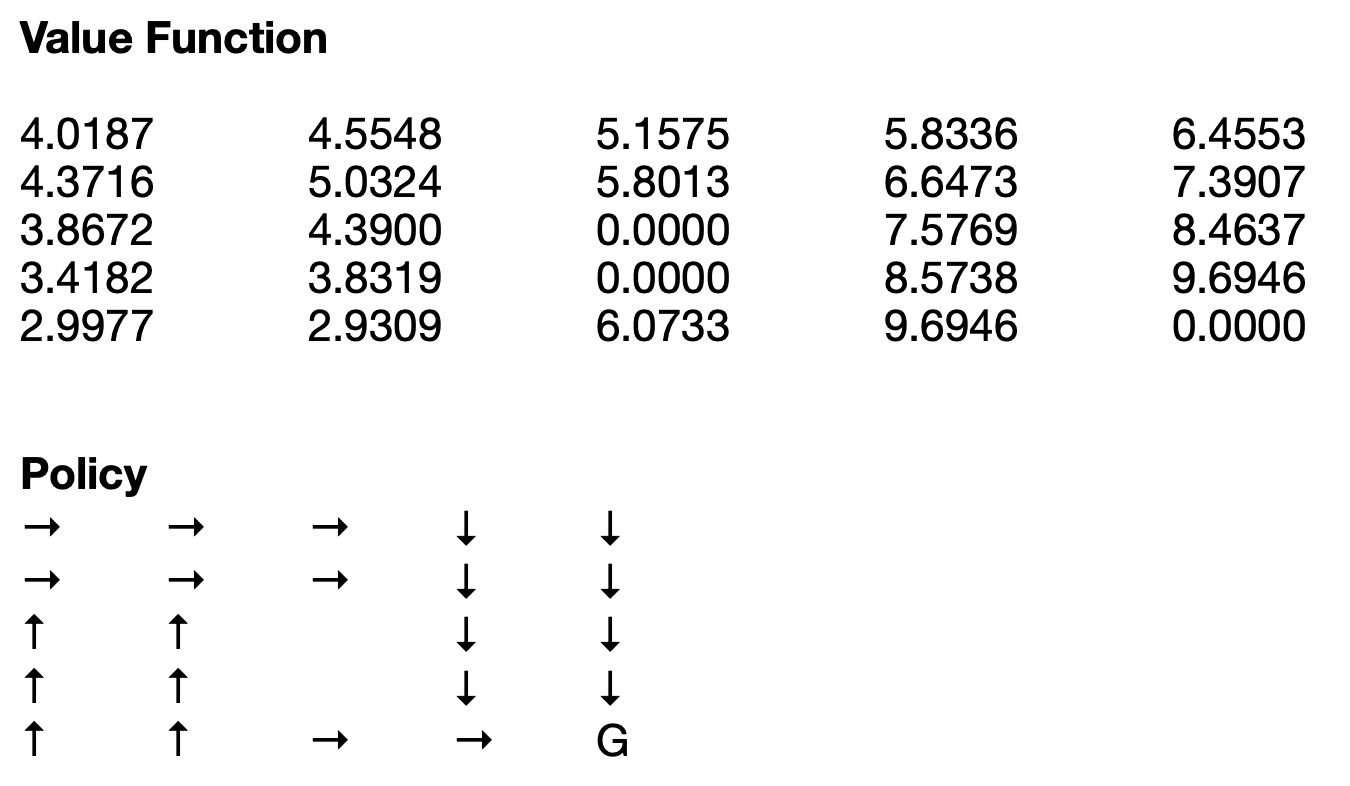
\includegraphics[width=0.55\textwidth]{HW_figs/v_pi_star_gridworld.png}
    \caption{Optimal value function and optimal policy for the 687-GridWorld domain.}
    \label{fig:v_pi_star}
\end{figure}

\vspace{0.6cm}

\begin{enumerate}
    \item {\Large{\textbf{TD-Learning on the 687-Gridworld} \POINTS{[20 Points, total]}}}
    
    First, implement the TD-Learning algorithm for policy evaluation and use it to construct an estimate, $\hat{v}$, of the value function of the optimal policy, $\pi^*$, for the 687-Gridworld. \textbf{Remember that both the optimal value function and optimal policy for the 687-Gridworld domain were identified in a previous homework by using the Value Iteration algorithm. For reference, both of them are shown in Figure \ref{fig:v_pi_star}.} When sampling trajectories, set $d_0$ to be a uniform distribution over $\mathcal{S}$ to ensure that you are collecting returns from all states. Do not let the agent be initialized in an Obstacle state. Notice that using this alternative definition of $d_0$ (instead of the original one) is important because we want to generate trajectories from all states of the MDP, not just states that are visited under the optimal deterministic policy shown in Figure \ref{fig:v_pi_star}. 
    
    \vspace{0.2cm}
    
    You should run your algorithm until the value function estimate does not change significantly between successive iterations; i.e., whenever the Max-Norm between $\hat{v}_{t-1}$ and $\hat{v}_t$ is at most $\delta$, for some value of $\delta$ that you should set empirically. For each run of your algorithm, count how many episodes were necessary for it to converge to an estimate of $v^{\pi^*}$. You should run your algorithm, as described above, 50 times and report: 
    \vspace{0.3cm}


        \textbf{(Question 1a.~\POINTS{2 Points})} the value of $\alpha$ that was used. You should pick a value of $\alpha$ that causes the algorithm to converge to a solution that is close to $v^{\pi^*}$, while not requiring an excessively large number of episodes.
        %
        % YOUR RESPONSE HERE
        %
        
        \textbf{(Question 1b.~\POINTS{9 Points})} the average value function estimated by the algorithm---i.e., the average of all 50 value functions learned by the algorithm at the end of its execution. Report, also, the Max-Norm between this average value function and the optimal value function for the 687-Gridworld domain.
        %
        % YOUR RESPONSE HERE
        %
        
        \textbf{(Question 1c.~\POINTS{9 Points})} the average and the standard deviation of the number of episodes needed for the algorithm to converge.
        %
        % YOUR RESPONSE HERE
        %
    
    
    
    \vspace{1.25cm}
    \item {\Large{\textbf{SARSA on the 687-Gridworld} \POINTS{[20 Points, total]}}} 
    
    Implement the SARSA algorithm and use it to construct $\hat{q}$, an estimate of the optimal \textbf{action-value function}, $q^{\pi^*}$, of the 687-Gridworld domain; and to construct an estimate, $\hat{\pi}$, of its optimal policy, $\pi^*$. You will have to make four main design decisions: \textit{(i)} which value of $\alpha$ to use; \textit{(ii)} how to initialize the $q$-function; you may, e.g., initialize it with zeros, with random values, or optimistically. Remember that $q(s_\infty, \cdot)=0$ by definition; \textit{(iii)} how to explore; you may use different exploration strategies, such as $\epsilon$-greedy exploration or softmax action selection; and \textit{(iv)} how to control the exploration rate over time; you might choose to keep the exploration parameter (e.g., $\epsilon$) fixed over time, or have it decay as a function of the number of episodes. 
    \vspace{0.3cm}
    
    
        \textbf{(Question 2a.~\POINTS{2 Points})} Report the design decisions \textit{(i, ii, iii, and iv)} you made and discuss what was the reasoning behind your choices.
        %
        % YOUR RESPONSE HERE
        %
        
        \textbf{(Question 2b.~\POINTS{7 Points})} Construct a learning curve where you show, on the $x$ axis, the total number of actions taken by the agent, from the beginning of the training process (i.e., the total number of steps taken across all episodes up to that moment in time). On the $y$ axis, you should show the number of episodes completed up to that point. If learning is successful, this graph should have an increasing slope, indicating that as the agent takes more and more actions (and thus executes more learning updates), it requires fewer actions/timesteps to complete each episode. Your graph should, ideally, look like the figure shown in Example 6.5 of the RL book (2nd edition). To construct this graph, run your algorithm 20 times and show the average curve across those runs.
        %
        % YOUR RESPONSE HERE
        %
        
        \textbf{(Question 2c.~\POINTS{8 Points})} Construct another learning curve: one where you show the number of episodes on the $x$ axis, and, on the $y$ axis, the mean squared error between your current estimate of the value function, $\hat{v}$, and the true optimal value function, $v^{\pi^*}$. The mean squared error between two value functions, $v_1$ and $v_2$, can be computed as $\frac{1}{|\mathcal{S}|}\sum_s (v_1(s) - v_2(s))^2$. Remember that SARSA estimates a $q$-function ($\hat{q}$), however, not a value function ($\hat{v}$). To compute $\hat{v}$, remember that $\hat{v}(s) = \sum_a \pi(s,a) \hat{q}(s,a)$. Remember, also, that the SARSA policy $\pi$, at each given moment, depends on your exploration strategy. Let us say, for example, that you are using $\epsilon$-greedy exploration. Then, in the general case when more than one action may be optimal with respect to $\hat{q}(s, a)$, the $\epsilon$-greedy policy would be as follows:
            \begin{equation}
            \pi(s,a) = \begin{cases}
            \frac{1-\epsilon}{|\mathcal A^*|} +  \frac{\epsilon}{|\mathcal A|} &\mbox{if } a \in \mathcal A^*\\
            \frac{\epsilon}{|\mathcal A|}&\mbox{otherwise,}
            \end{cases}
        \end{equation} 
    \noindent where $\mathcal A^* = \arg\max_{a \in \mathcal A}\hat{q}(s,a)$. To construct the learning curve, run your algorithm 20 times and show the average curve across those runs; i.e., the average mean squared error, computed over 20 runs, as a function of the number of episodes.
    %
    % YOUR RESPONSE HERE
    %
        
    \textbf{(Question 2d.~\POINTS{3 Points})} Show the \textit{greedy policy} with respect to the $q$-values learned by SARSA.
    %
    % YOUR RESPONSE HERE
    %
    
    
    
    \vspace{1.cm}
    \item {\Large{\textbf{Q-Learning on the 687-Gridworld}} \POINTS{[20 Points, total]}} 
    
    
    Answer the same questions as above (\textit{2a, 2b, 2c, and 2d}), but now using the Q-Learning algorithm; i.e., you will be using Q-Learning to solve the 687-Gridworld domain. When computing $\hat{v}$, for question \textit{3c}, you should compute the value function of the greedy policy: $\hat{v}(s) = \max_a \hat{q}(s,a)$. The amount of points associated with questions \textit{3a, 3b, 3c, and 3d}, will be the same as those associated with the corresponding items of Question 2.
    %
    % YOUR RESPONSE HERE
    %
    
    
    
    \vspace{1.cm}
    \item {\Large{\textbf{SARSA on the Mountain Car domain} \POINTS{[20 Points, total]}}} 
    
    You will now use the SARSA algorithm to solve the Mountain Car domain. Notice that in the Mountain Car domain, states are continuous. You will first have to discretize them in order to be able to deploy the standard/tabular version of SARSA\footnote{Suppose you are discretizing a continuous state $s=[x,v]$, where the range of $x$ is $[-1.2, 0.5]$ and the range of $v$ is $[-0.07, 0.07]$. Suppose you choose to discretize each component of the state into 3 bins. To do so, you will break down the interval of values of $x$ (from $-1.2$ to $0.5$) into three contiguous bins: the first bin would correspond to values of $x$ from $-1.2$ to $-0.634$; the second bin would correspond to values of $x$ from $-0.634$ to $-0.068$; and the third bin, to values of $x$ from $-0.068$ to $0.5$. You would perform a similar discretization process over the state variable $v$. Then, the final  discretized version of a continuous state $s=[x,v]$ would correspond to a pair $(b_x, b_v)$ indicating the number of the bin, $b_x$, on which the $x$ variable fell; and the number of the bin, $b_v$, where the $v$ variable fell. Notice that if you discretize a 2-dimensional continuous state (such as that of the Mountain Car domain) into $N$ bins, you will end up with $N^2$ discrete states. Using a coarser discretization results in fewer states, but where each discrete state is a ``less accurate'' representation of the true underlying continuous state. Using a finer discretization results in a ``more accurate'' representation of the true underlying continuous state, but generates a larger state space.}. You will have to make five main design decisions, here: the same four design decisions as in Question 2, and also an additional design decision (design decision \textit{v}): the level of discretization to be used; i.e., the number of bins used to discretize the continuous state of the MDP.
    \vspace{0.3cm}
    
        \textbf{(Question 4a.~\POINTS{2 Points})} Report the design decisions \textit{(i, ii, iii, iv, and v)} you made and discuss what was the reasoning behind your choices.
        %
        % YOUR RESPONSE HERE
        %
        
        \textbf{(Question 4b.~\POINTS{9 Points})} Construct a learning curve where you show, on the $x$ axis, the total number of actions taken by the agent, from the beginning of the training process (i.e., the total number of steps taken across all episodes up to that moment in time). On the $y$ axis, you should show the number of episodes completed up to that point. If learning is successful, this graph should have an increasing slope, indicating that as the agent takes more and more actions (and thus executes more learning updates), it requires fewer actions/timesteps to complete each episode. Your graph should, ideally, look like the figure shown in Example 6.5 of the RL book (2nd edition). To construct this graph, run your algorithm 20 times and show the average curve across those runs.
        %
        % YOUR RESPONSE HERE
        %

        \textbf{(Question 4c.~\POINTS{9 Points})} Construct another learning curve: one where you show the number of episodes on the $x$ axis, and, on the $y$ axis, the number of steps needed by the agent to reach the goal state. To construct this graph, run your algorithm 20 times and show the average curve across those runs (i.e., the average number of steps to reach the goal, computed across 20 runs, as a function of the number of episodes). Show, also, the standard deviation associated with each of these points. Your graph should, ideally, look like that in Figure \ref{fig:example_plot}.
        %
        % YOUR RESPONSE HERE
        %    
        
        
    \begin{figure}[!hb]
    \centering
    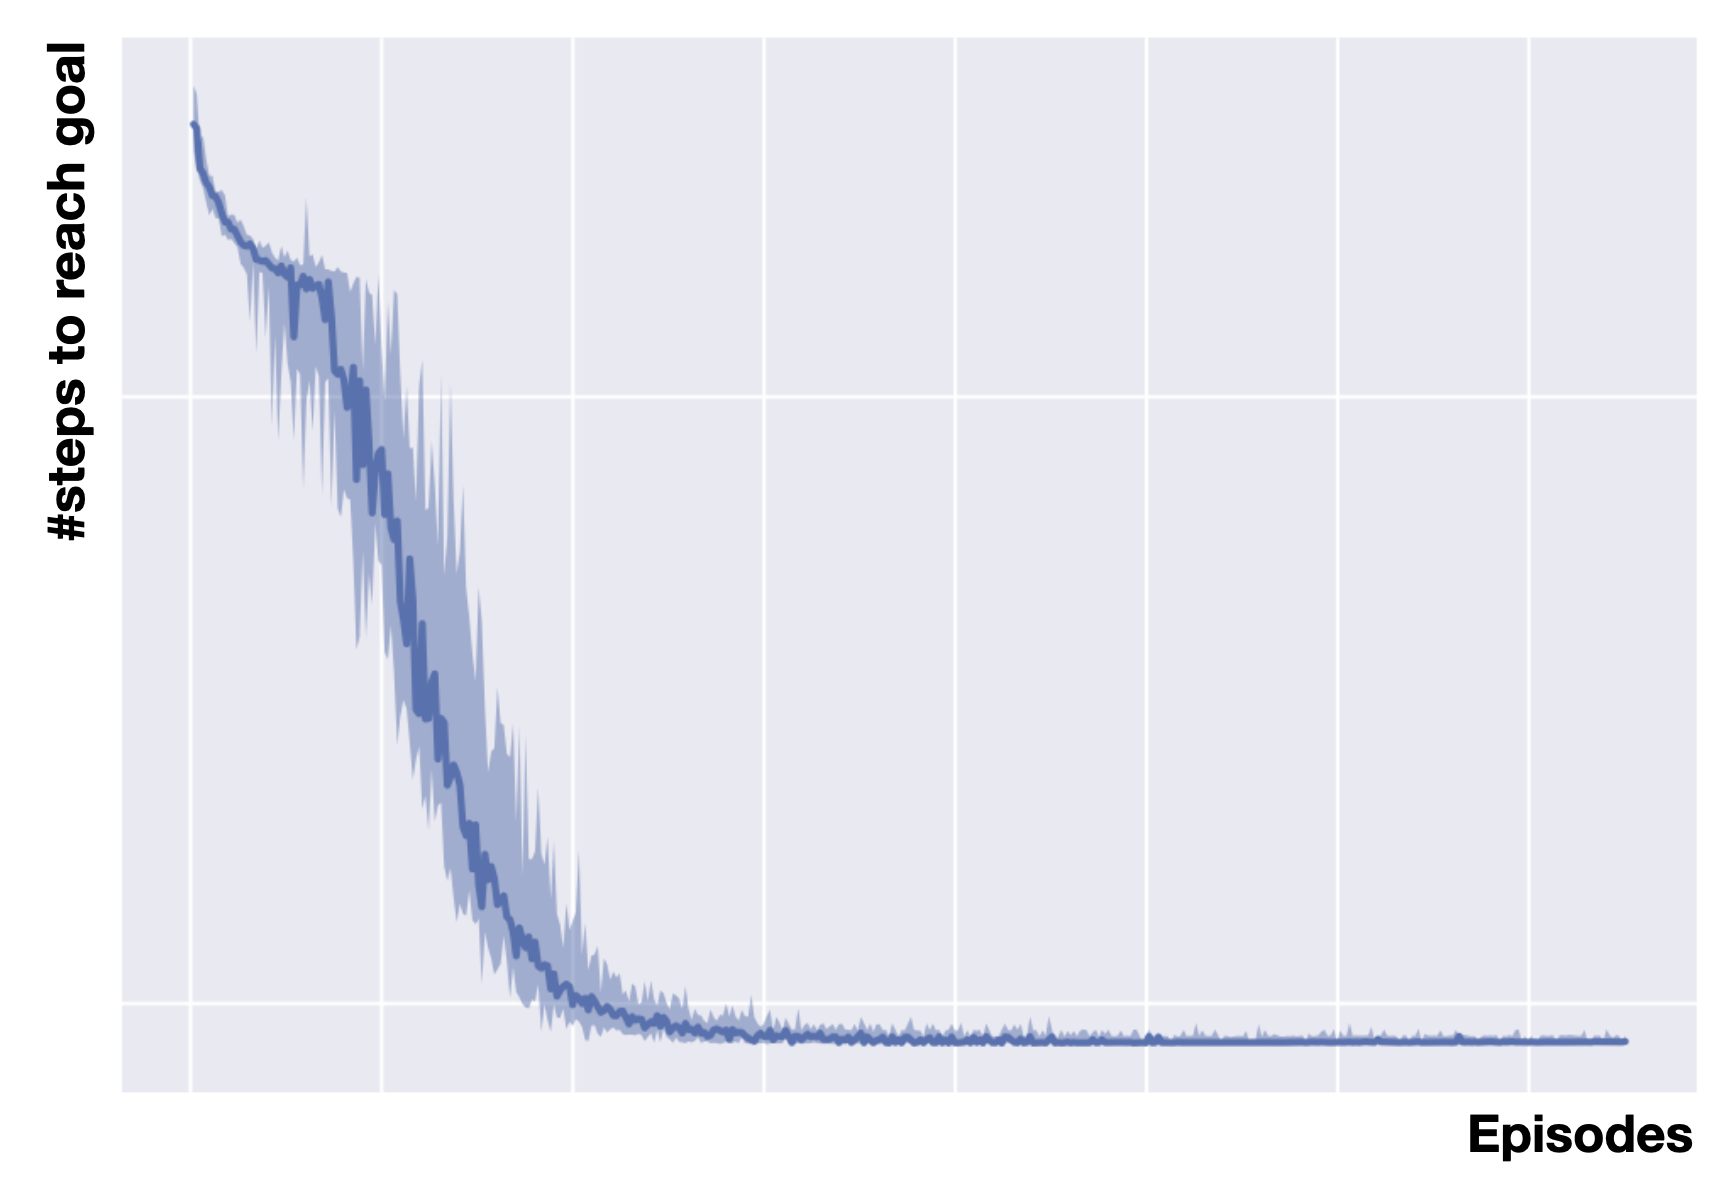
\includegraphics[width=0.5\textwidth]{HW_figs/example_graph.png}
    \caption{Example of a learning curve: average number of steps to reach the goal (and the associated standard deviation) as a function of the number of episodes.}
    \label{fig:example_plot}
\end{figure}
        
        
        
    \vspace{1cm}    
    \item {\Large{\textbf{Q-Learning on the Mountain Car domain} \POINTS{[20 Points, total]}}}
    
    
    Answer the same questions as above (\textit{4a, 4b, and 4c}), but now using the Q-Learning algorithm; i.e., you will be using Q-Learning to solve the Mountain Car domain. The amount of points associated with questions \textit{5a, 5b, and 5c}, will be the same as those associated with the corresponding items of Question 4.
    %
    % YOUR RESPONSE HERE
    %


\newpage
\vspace{0.5cm}
\noindent\rule{\textwidth}{1pt}
\vspace{0.25cm}

\item {\Large{\textbf{Extra Credit} \POINTS{[16 Points, total]}}} 
\vspace{0.25cm}

\textbf{(Question 6a.~\POINTS{8 Points})} Answer questions \textit{(4b)} and \textit{(4c)} once again, but now using different discretization levels compared to the one you selected when solving Question 4. In particular, you should use the same hyperparameters as in Question 4: same value of $\alpha$, $q$-function initialization strategy, exploration strategy, and method for controlling the exploration rate over time. Now, however, you will experiment with \textit{different} discretization levels compared to the one you selected when solving Question 4. You should, in particular, run experiments with 25\% fewer bins, 50\% fewer bins, 25\% more bins, and 50\% more bins. Let us say, for example, that in Question 4 you decided to discretize the state features into $N$ bins. In this extra-credit question, you should run the same  experiments as in \textit{(4b)} and \textit{(4c)}, but now using $0.5N$ bins, $0.75N$ bins, $1.25N$ bins, and $1.5N$ bins. Discuss the impact that each of these alternative discretization schemes had both on the performance of the policy learned by the algorithm, and on the (wall-clock) time needed to complete each of the four experiments, compared to the wall-clock time required to run the corresponding experiment in Question 4.
    %
    % YOUR RESPONSE HERE
    %



\vspace{0.25cm}
\textbf{(Question 6b.~\POINTS{8 Points})} Answer questions \textit{(4b)} and \textit{(4c)} once again, but now using \textit{two} different ways of initializing the $q$-function optimistically. You should use the same hyperparameters as in Question 4: same value of $\alpha$ and discretization levels. Now, however, you will experiment with \textit{different} ways of optimistically initializing the $q$-function. Let $M$ be the maximum return achievable in Mountain Car. First, deterministically initialize all entries of the $q$-function with the optimistic value $2M$. Next, stochastically initialize all entries of the $q$-function with numbers drawn uniformly at random from the interval $[1.5M, 3.5M]$. In this extra-credit question, you should run the same experiments as in \textit{(4b)} and \textit{(4c)}, but now using these alternative ways of optimistically initializing the $q$-function. \textbf{Importantly, when running these experiments you should set the exploration rate to zero (i.e., $\epsilon=0$, always)}. Discuss the impact that these $q$-function initialization strategies had both on the performance of the policy learned by the algorithm, and on the (wall-clock) time needed to complete each of the four experiments, compared to the wall-clock time required to run the corresponding experiment in Question 4.
    %
    % YOUR RESPONSE HERE
    %
    
    
    
\end{enumerate}
\end{document}



    
    
